\section{Comparing the accuracy of CRKs to HBs}
\label{section:crks_vs_hbs}

\subsection{hb6, hb8, hb10 vs crk65}

\paragraph{Problem 1} We can see in Figures $\ref{fig:discrete_crk65_vs_hbs_p1_5}$ and $\ref{fig:discrete_crk65_vs_hbs_p1_10}$ that at lower tolerances, HB6 is worse than HB8 and HB10 but HB10 seems to not be much better than HB8. However at sharper tolerances, HB10 performs better. This is because though HB10 has higher order, that is just a big O analysis. The coefficient for that analysis for HB10 is bigger than that for HB8. We also note that this is as expected as there is another multiplier in the actual error term as HB10 is technically over one more step. We note that the interpolants from CRK65 are more accurate than the HB interpolants.

\begin{figure}[H]
\centering
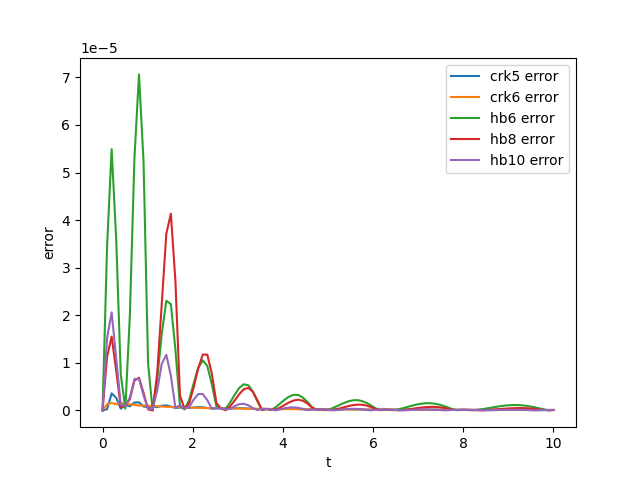
\includegraphics[width=0.7\linewidth]{./figures/discrete_crk65_vs_hbs_p1_5}
\caption{Discrete error control crk65 plotted alongside HB6, Hb8, HB10 with Problem 1 at a tolerance of $10^{-5}$.}
\label{fig:discrete_crk65_vs_hbs_p1_5}
\end{figure}

\begin{figure}[H]
\centering
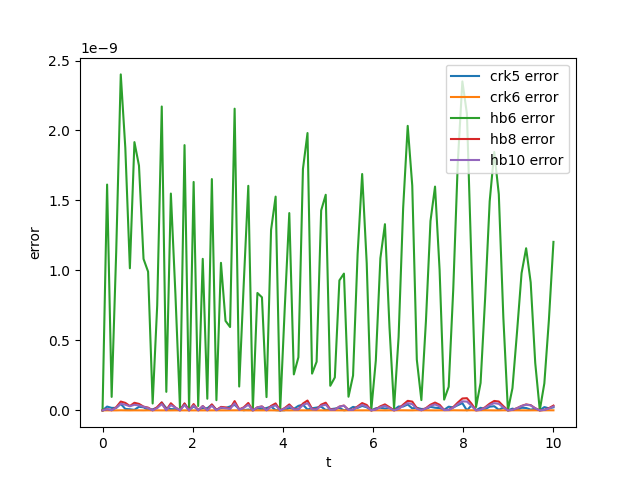
\includegraphics[width=0.7\linewidth]{./figures/discrete_crk65_vs_hbs_p1_10}
\caption{Discrete error control crk65 plotted alongside HB6, Hb8, HB10 with Problem 1 at a tolerance of $10^{-10}$.}
\label{fig:discrete_crk65_vs_hbs_p1_10}
\end{figure}

\paragraph{Problem 2} We can see in Figures $\ref{fig:discrete_crk65_vs_hbs_p2_5}$ and $\ref{fig:discrete_crk65_vs_hbs_p2_10}$ that at lower tolerances, HB6 is worse than HB8 and HB10 but HB10 seems to not be much better than HB8. However at sharper tolerances, HB10 performs better. This is because though HB10 has higher order, that is just a big O analysis. The coefficient for that analysis for HB10 is bigger than that for HB8. We also note that this is as expected as there is another multiplier in the actual error term as HB10 is technically over one more step. 


\begin{figure}[H]
\centering
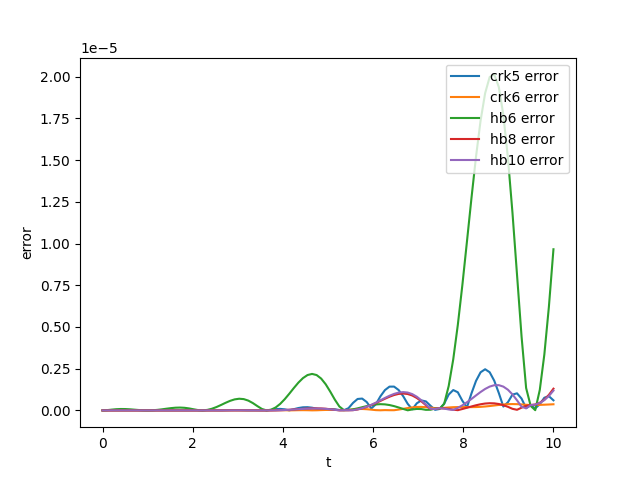
\includegraphics[width=0.7\linewidth]{./figures/discrete_crk65_vs_hbs_p2_5}
\caption{Discrete error control crk65 plotted alongside HB6, Hb8, HB10 with Problem 2 at a tolerance of $10^{-5}$.}
\label{fig:discrete_crk65_vs_hbs_p2_5}
\end{figure}

\begin{figure}[H]
\centering
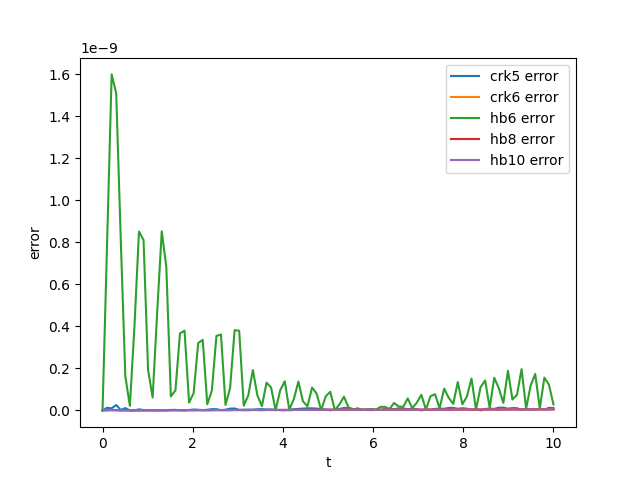
\includegraphics[width=0.7\linewidth]{./figures/discrete_crk65_vs_hbs_p2_10}
\caption{Discrete error control crk65 plotted alongside HB6, Hb8, HB10 with Problem 2 at a tolerance of $10^{-10}$.}
\label{fig:discrete_crk65_vs_hbs_p2_10}
\end{figure}

\paragraph{Problem 3} We can see in Figures $\ref{fig:discrete_crk65_vs_hbs_p3_5}$ and $\ref{fig:discrete_crk65_vs_hbs_p3_10}$ that at lower tolerances, HB6 is worse than HB8 and HB10 but HB10 seems to not be much better than HB8. However at sharper tolerances, HB10 performs better. This is because though HB10 has higher order, that is just a big O analysis. The coefficient for that analysis for HB10 is bigger than that for HB8. We also note that this is as expected as there is another multiplier in the actual error term as HB10 is technically over one more step. 


\begin{figure}[H]
\centering
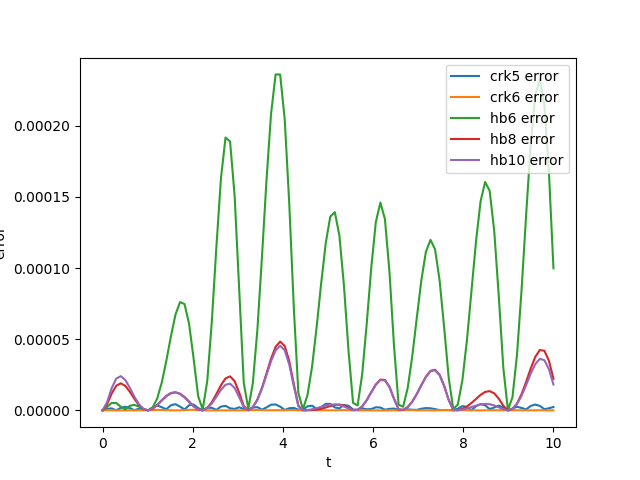
\includegraphics[width=0.7\linewidth]{./figures/discrete_crk65_vs_hbs_p3_5}
\caption{Discrete error control crk65 plotted alongside HB6, Hb8, HB10 with Problem 3 at a tolerance of $10^{-5}$.}
\label{fig:discrete_crk65_vs_hbs_p3_5}
\end{figure}

\begin{figure}[H]
\centering
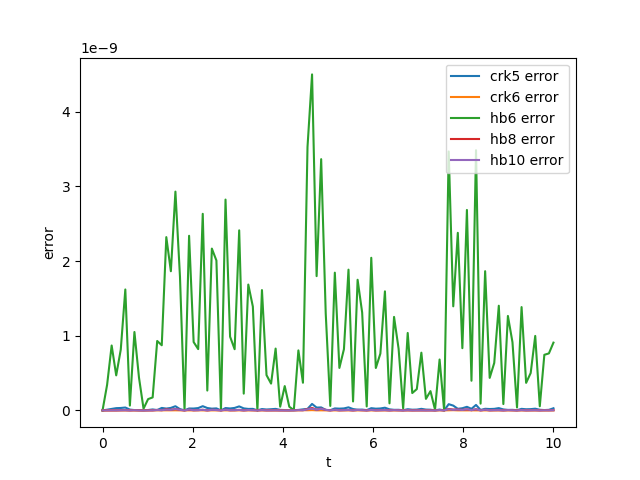
\includegraphics[width=0.7\linewidth]{./figures/discrete_crk65_vs_hbs_p3_10}
\caption{Discrete error control crk65 plotted alongside HB6, Hb8, HB10 with Problem 3 at a tolerance of $10^{-10}$.}
\label{fig:discrete_crk65_vs_hbs_p3_10}
\end{figure}

\subsection{hb8, hb10 vs crk87}

\paragraph{Problem 1} In this comparison in Figures $\ref{fig:discrete_crk87_vs_hbs_p1_5}$ and $\ref{fig:discrete_crk87_vs_hbs_p1_10}$ between HB8 and HB10 fitted onto data provided by the CRK87, we can more clearly see that HB8 is more accurate at lower tolerances but HB10 is more accurate at the sharper tolerance. This is because of the error term having one additional multiplier and thus though the big O analysis say that HB10 is of higher order, it has a bigger coefficient.

\begin{figure}[H]
\centering
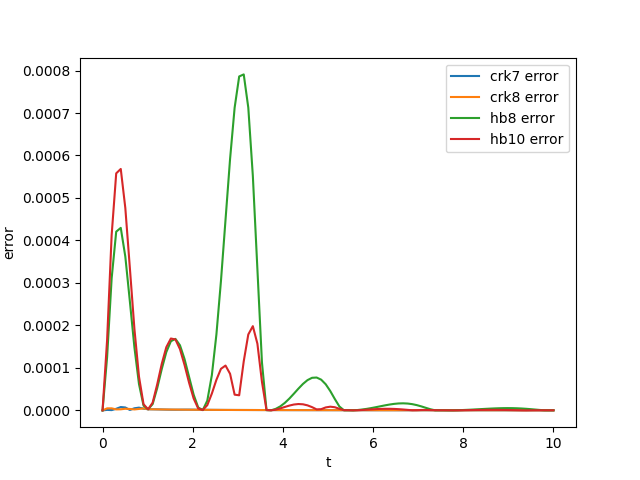
\includegraphics[width=0.7\linewidth]{./figures/discrete_crk87_vs_hbs_p1_5}
\caption{Discrete error control crk87 plotted alongside Hb8, HB10 with Problem 1 at a tolerance of $10^{-5}$.}
\label{fig:discrete_crk87_vs_hbs_p1_5}
\end{figure}

\begin{figure}[H]
\centering
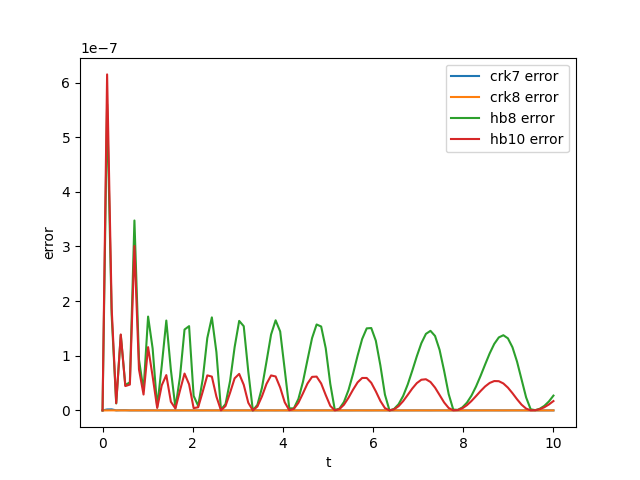
\includegraphics[width=0.7\linewidth]{./figures/discrete_crk87_vs_hbs_p1_10}
\caption{Discrete error control crk87 plotted alongside Hb8, HB10 with Problem 1 at a tolerance of $10^{-10}$.}
\label{fig:discrete_crk87_vs_hbs_p1_10}
\end{figure}

\paragraph{Problem 2} In this comparison in Figures $\ref{fig:discrete_crk87_vs_hbs_p2_5}$ and $\ref{fig:discrete_crk87_vs_hbs_p2_10}$ between HB8 and HB10 fitted onto data provided by the CRK87, we can more clearly see that HB8 is more accurate at lower tolerances but HB10 is more accurate at the sharper tolerance. This is because of the error term having one additional multiplier and thus though the big O analysis say that HB10 is of higher order, it has a bigger coefficient.

\begin{figure}[H]
\centering
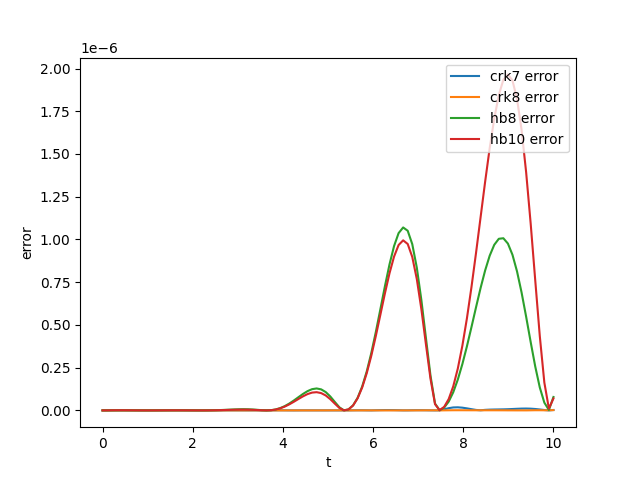
\includegraphics[width=0.7\linewidth]{./figures/discrete_crk87_vs_hbs_p2_5}
\caption{Discrete error control crk87 plotted alongside  Hb8, HB10 with Problem 2 at a tolerance of $10^{-5}$.}
\label{fig:discrete_crk87_vs_hbs_p2_5}
\end{figure}

\begin{figure}[H]
\centering
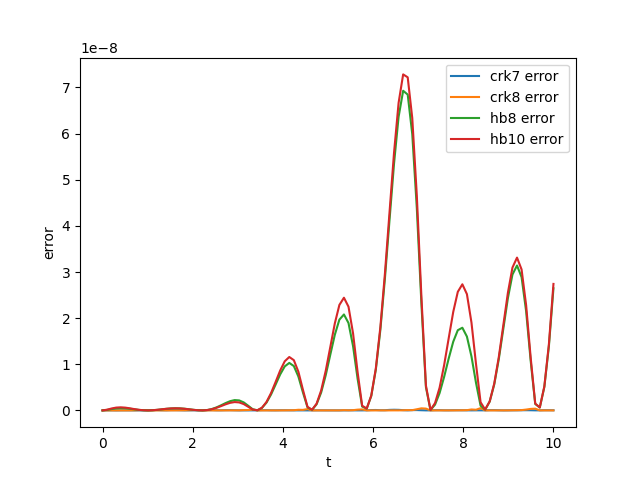
\includegraphics[width=0.7\linewidth]{./figures/discrete_crk87_vs_hbs_p2_10}
\caption{Discrete error control crk87 plotted alongside Hb8, HB10 with Problem 2 at a tolerance of $10^{-10}$.}
\label{fig:discrete_crk87_vs_hbs_p2_10}
\end{figure}

\paragraph{Problem 3} In this comparison in Figures $\ref{fig:discrete_crk87_vs_hbs_p3_5}$ and $\ref{fig:discrete_crk87_vs_hbs_p3_10}$ between HB8 and HB10 fitted onto data provided by the CRK87, we can more clearly see that HB8 is more accurate at lower tolerances but HB10 is more accurate at the sharper tolerance. This is because of the error term having one additional multiplier and thus though the big O analysis say that HB10 is of higher order, it has a bigger coefficient.

\begin{figure}[H]
\centering
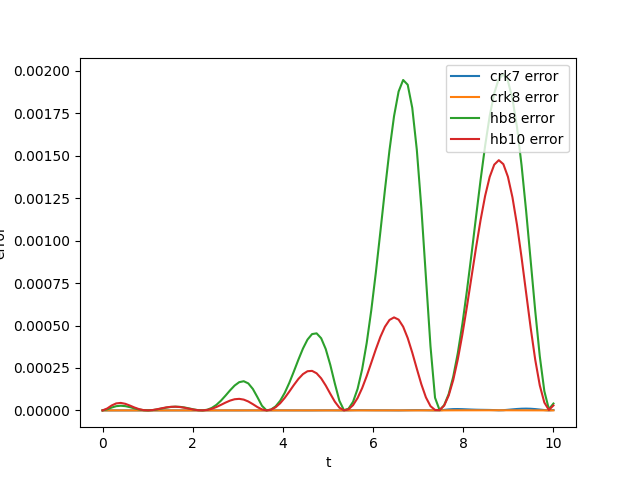
\includegraphics[width=0.7\linewidth]{./figures/discrete_crk87_vs_hbs_p3_5}
\caption{Discrete error control crk87 plotted alongside Hb8, HB10 with Problem 3 at a tolerance of $10^{-5}$.}
\label{fig:discrete_crk87_vs_hbs_p3_5}
\end{figure}

\begin{figure}[H]
\centering
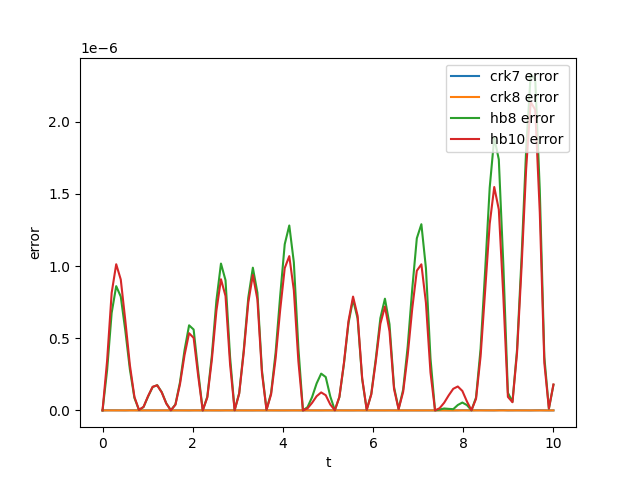
\includegraphics[width=0.7\linewidth]{./figures/discrete_crk87_vs_hbs_p3_10}
\caption{Discrete error control crk87 plotted alongside Hb8, HB10 with Problem 3 at a tolerance of $10^{-10}$.}
\label{fig:discrete_crk87_vs_hbs_p3_10}
\end{figure}